% !TEX root = ../main.tex

%=========================================================
\chapter{\label{chapitre:caracterisation} Caractériser les comportements mémoires}
%=========================================================

%% Our microbenchmarks have shown that applications may exhibit a wide
%% variety of behavior depending on the nature and the intensity of their
%% memory consumption.  However, we have not characterized this
%% consumption otherwise than by the microbenchmarks' parameters.

%% \minitoc

Dans le chapitre précédent, nous avons introduit un ensemble de microbenchmarks pour étudier l'impact des interférences sur les applications selon leur comportement d'accès à la mémoire.
Nous avons, alors, caractérisé le comportement des microbenchmarks en fonction de leur paramètre.
Ces paramètres ne régissant que le comportement de nos microbenchmarks, les résultats de cette étude ne sont donc pas directement transposables à des applications quelconques.
Pour remédier à ce problème, nous devons quantifier les aspects pertinents du comportement mémoire en ce qui concerne la sensibilité aux interférences.
De notre caractérisation événementielle de l'activité mémoire, nous avons pu distinguer des aspects liés à la nature et à la sensibilité des applications.
De cette dichotomie, nous pouvons tirer deux grands groupes de métriques caractérisant l'activité mémoire: les \emph{métriques quantitatives} décrivant les aspects liés à l'intensité du trafic et les \emph{métriques qualitatives} liées à sa nature.

Les métriques quantitatives sont en général mesurables simplement en employant des compteurs matériels de performances.
Ce n'est malheureusement pas le cas pour la plupart des métriques qualitatives.
Nous contournerons cette limitation en utilisant le modèle événementiel décrit dans le chapitre précédent pour implanter un outil de profilage.
Afin de contourner ce problème, nous nous baserons sur le modèle événementiel décrit dans le chapitre précédent pour implanter un outil de capture de profil haute résolu
En plus d'être utiles pour mesurer de nouvelles métriques, nous montrerons que cet outil peut être utilisé pour générer des profils en haute résolution de l'activité mémoire des applications, qui révèlent les différentes phases dans l'exécution de ces dernières.

Le reste de chapitre est organisé de la façon suivante.
En premier lieu, nous traitons de la caractérisation quantitative de l'utilisation de la mémoire.
En deuxième lieu, nous nous penchons sur la caractérisation des aspects qualitatifs du trafic mémoire.
En troisième et dernier lieu, nous présenterons notre solution de profilage.


% The rest of this section is organized as follows.
% In the first place, we study the quantitative characterization of memory behavior using bandwidth.
% In a second place, based on our previous results and our knowledge of the experimental platform we propose some qualitative metrics.
% In a third place, we present our profiling platform, and our high resolution profile.
% We conclude this section with a case study of an application from the \textsc{PARSEC} suite.

\section{\label{subsection:quantitative} Caractérisation quantitative par la bande passante}

La caractérisation quantitative décrit la quantité de requêtes d'accès généré par une application.
Dans la section~\ref{section:eval-microbenchmarks} du chapitre précédent, l'aspect quantitatif du comportement d'accès d'un microbenchmark est contrôlé par le paramètre $F$, décrivant l'espacement entre les requêtes en lecture et celles en écritures.
Pour mesurer l'utilisation quantitative du système mémoire, il est courant d'utiliser la \emph{bande passante}. 
La bande passante $BW$ d'une application est le nombre d'accès $N_{access}$ effectué sur une durée $T$.

$$ BW = \frac{N_{Access}}{T} $$

%Dans le cadre de l'analyse d'interférences, il s'agit d'une caractéristique importante, car elle permet de quantifier la sollicitation par un programme de ressources matérielles partagées.
Il s'agit d'une grandeur importante pour l'analyse d'interférences, car elle quantifie la fréquence d'accès à la mémoire.
Une bande passante élevée impliquant une importante sollicitation des ressources partagées dans le temps, elle indique une grande agressivité sur celles-ci.
Paradoxalement, elle indique également une grande sensibilité au problème des interférences.
On peut, en effet, directement exprimer le surcoût temporel subi par une application en fonction de sa bande passante.
En notant $D_{access}$ le retard moyen subi par accès, on peut exprimer le retard total ainsi : 

\begin{equation}
	\begin{split}
		D_{total} &= T_{cont} - T{iso} \\
				  &= N_{access} * D_{access} \\
	\end{split}
\end{equation}

En divisant cette expression par le temps d'exécution en isolation, on peut lier la bande passante avec le facteur de ralentissement subi.

\begin{equation}
	\begin{split}
	 \frac{D_{total}}{T_{iso}} &= \frac{T_{cont} - T_{iso}}{T_{iso}} \\
	 						   &= \frac{N_{access} * D_{access}}{T} \\
	  \Leftrightarrow Overhead &= BW \cdot D_{access}
	\end{split}
	 \label{eq:o_bw_daccess}
\end{equation}

La bande passante n'exprime donc pas seulement à quelle fréquence les requêtes d'accès sont émises, mais aussi à quelle fréquence le retard subi en moyenne par chaque accès est propagé dans le temps d'exécution en contention.
Le retard subi par une application est donc linéairement croissant en fonction de la bande passante de cette dernière.
La vitesse à laquelle le retard croît est donnée par $D_{access}$.
Cette quantité nous permet donc d'étudier le retard subi indépendamment de la consommation mémoire.

Sur les architectures modernes, la bande passante peut se mesurer assez facilement à l'aide de compteurs matériels de performance.
La diversité des points de mesures pose néanmoins la question du choix de quel composant de la hiérarchie mémoire considéré pour la mesure.
Sur notre plateforme, nous avons identifié deux mémoires sujettes aux interférences: le cache L2 sujet à des interférences temporelles et la mémoire principale sujettes à des interférences spatiales \emph{et} temporelles.
Notre carte nous permet de mesurer la bande passante vers ces deux composants:
\begin{itemize}
	\item La bande passante vers la mémoire principale (notée $BW^{DRAM}$) est mesurée à l'aide de la PMU situé dans le $MMDC$ de notre carte.
	\item La bande passante vers le cache L2 (notée $BW^{L2}$) est mesurée à l'aide du compteur de défauts de cache L1 fourni par la PMU du cœur exécutant l'application.
\end{itemize}

Le partage ou non des points de mesures ont une influence sur ce que l'on peut mesurer.
La bande passante vers la mémoire principale se mesure à l'aide d'une PMU situé dans le contrôleur mémoire, dont les compteurs enregistrent le trafic émis par tous les cœurs en même temps.
On ne peut donc pas quantifier la part individuelle de chaque cœur dans le trafic enregistré.
La bande passante vers la mémoire principale ne peut donc être enregistrée qu'en isolation.
Ce qui n'est pas un problème pour la caractérisation de comportement.
Cette limitation n'existe pas pour la bande passante vers le cache L2.
Dans tous les cas, lorsque nous parlerons de bande passante il sera sous-entendu bande passante \emph{en isolation}.

Prise séparément, chacune de ces bandes passantes ne peut exprimer qu'une portion du trafic au sein du système mémoire.
Dans le cas de la mémoire principale, la bande passante vers ce composant est une mesure du débit d'accès ayant traversé toute la hiérarchie mémoire.
Une incertitude demeure sur les accès n'ayant traversé que partiellement la hiérarchie.
Sur notre carte, c'est le cas des défauts de cache L1 n'ayant pas entraîné de défaut de cache L2.
Réciproquement, la bande passante vers le cache L2 ne capture pas l'activité pour les composants situés après celui-ci.
Cette incertitude est une limitation pour les systèmes de régulation basés sur la bande passante.
MemGuard~\cite{yun2013memguard} utilise la bande passante vers le cache L2, tandis que Blin et al.~\cite{blin2016maximizing} utilisent la bande passante vers la mémoire principale.

% Nous mesurons deux bande passantes différentes: celle à destination de la mémoire principale, et celle à destination du cache de niveau 2.
% \begin{itemize}
% 	\item La bande passante vers la mémoire principale est une mesure de la bande passante vers la mémoire partagée.
% 	Un accès émis vers la mémoire principale ayant traversé toute la hiérarchie mémoire, cette bande passante est une mesure de bout en bout de la consommation mémoire.
% 	Nous la mesurons à l'aide des compteurs matériels situés dans la PMU du controleur DRAM de notre plateforme.
% 	Nous rappelons que ces compteurs sont communs à tout les coeurs, et que l'on ne peut pas discriminer le traffic émis par les différents coeurs.
% 	La bande passante vers la mémoire principale d'une application ne peut donc être déterminé qu'en isolation.
% 	\item La bande passante vers le cache de niveau deux permet de mesurer la pression exercées sur le contrôleur de cache L2.
% 	Contrairement à la bande passante vers la mémoire principale, il ne s'agit pas d'une mesure de bout en bout de la consommation.
% 	Un accès vers le cache L2 n'entrainant pas forcément d'accès vers la mémoire principale.
% 	Rappelons par ailleurs que dans notre configuration, le cache de niveau 2 n'est pas partitionné, la contention est donc localisé au niveau du controleur PL310 et de la SCU.
% 	Cette bande passante est mesurée à l'aide de l'unité de la PMU situé dans chaque coeur Cortex A9.
% 	Il est donc possible de la déterminer aussi bien en isolation qu'en contention.
% \end{itemize}

% \subsection{Intensité}

% Dans le chapitre précedent, nous avons pu confirmer que l'intensité du trafic mémoire est une composante fondamentale de la sensibilité d'un programme au programme aux interférences.
% Nous caractérisons l'intensité du traffic mémoire à l'aide de la bande passante vers la mémoire partagée.
% Il s'agit d'un choix relativement commun, qui est fait notamment dans les systèmes de régulation tel que l'approche de Blin et al.~\cite{blin2016maximizing} et MemGuard~\cite{yun2013memguard}.
% Nous la mesurons à l'aide des compteurs fournis par la PMU située dans le MMDC.
% Notons que ces compteurs sont communs à tout les coeurs.
% Cela signifie, que le traffic mesuré par ces compteurs est un \emph{trafic global}, et qu'il n'est pas possible de mesurer la consommation individuelle de chaque coeurs par ce moyen.
% C'est pourquoi, sauf mention contraire, nous entendrons par bande passante la bande passante d'une application en isolation, c'est à dire exécutée seul.
% Ce n'est heuresement pas un problème pour le type de caractérisation que nous souhaitons éffectuer.

% La figure~\ref{fig:bw_overhead} illustre le lien entre le retards subi par les instances de microbenchmarks que nous avons présenté dans le chapitre précedent et leur bande passante en isolation.
% Comme dans la figure~\ref{fig:throttle_overhead}, nous pouvons associer une courbe à chaque nature de traffic observée.
% Cette fois ci, les courbes montre une relation linéaire entre le retard subi et la bande passante en isolation.
% On y observe une forte variation dans la pente de ces courbes.
% On peut montrer que la pente de ces courbes est en fait le \emph{retard moyen subi par accès}.
% En effet, le retards moyen par accès est la différence entre la latence moyenne par accès en situation de contention et en isolation.

% \begin{equation}
% 	\label{equation:d_access}
% 	D_{access} = CPI_{mem}^{cont} - CPI_{mem}^{iso}
% \end{equation}

% Vu qu'il s'agit d'une valeur moyenne, on peut dire que le retards total subi est le retards moyen subi par accès subi $N_access$ fois.

% \begin{equation}
% 	\label{equation:degradation}
% 	T_{cont} - T_{iso} = N_{access} \cdot D_{access}
% \end{equation}

% En injectant ce résultat dans l'équation~\ref{equation:overhead}, on peut alors exprimer le facteur de ralentissement subi en fonction de la bande passante en isolation. 

% \begin{equation}
% 	\label{equation:overhead_bw_iso}
% 	\begin{split}
% 		Overhead & = \frac{T_{iso} - T_{cont}}{T_{iso}} \\
% 				 & = \frac{N_{access}}{T_{iso}} \cdot D_{access} \\
% 				 & = BW_{iso} \cdot {D_{access}} \\
% 	\end{split}
% \end{equation}

% On peut ainsi déduire le retards moyen subi par accès à partir du facteur de ralentissement et de la bande passante en isolation.
% Cette pente nous permet de raisonner sur la sensibilité d'une application indépendamment de sa bande passante.
% La figure~\ref{fig:throttle_racc} illustre la relation entre le facteur d'inhibition des microbenchmarks et le retards moyen subi par accès.
% On peut y voir que la pente associée à chaque nature de traffic est quasiment constante, mis à part deux exceptions notables : les valeurs de pentes élevés (plus de 200 cycles) sont relativement instables, et on peut obsever une baisse de sensibilité pour les valeurs élevé du facteur d'inhibition.
% Si on applique la formule~\ref{equation:overhead_bw_iso} en utisant les valeurs de pentes et de bande passante observées les plus importantes (respectivement 481,51 cycles par accès et 0,084 accès par cycles), on obtient alors un facteur de ralentissement de 40,74.
% Heureusement, nous pouvons observer, dans la figure~\ref{fig:bw_racc}, une apparente relation inverse entre la bande passante et la plus grosse pente observée, ce qui nous permet de penser que ce pire cas est en fait fort improbable.
% Nous pouvons en conclure de la nécessité de caractériser d'autre aspects du traffic mémoire.

% \begin{figure}[H]
% 	\centering
% 	%\begin{subfigure}[t]{0.4\textwidth}
% 	%	\includegraphics[width=\textwidth]{figures/throttle_bw.pdf}
% 	%	\caption{\label{fig:throttle_bw}}
% 	%\end{subfigure    \centering
% 	\begin{subfigure}[t]{0.48\linewidth}
% 	%\captionsetup{width=.8\linewidth
% 		\includegraphics[width=0.95\textwidth]{figures/bw_overhead.pdf}
% 		\caption{\label{fig:bw_overhead}Bandwidth in isolation vs. overhead (each point represents a microbenchmark instance)}
% 	\end{subfigure}
% 	\begin{subfigure}[t]{0.48\linewidth}
% 		\includegraphics[width=0.95\textwidth]{figures/throttle_racc.pdf}
% 		\caption{\label{fig:throttle_racc}Throttle rate vs average delay per access}
% 	\end{subfigure}
% 	\begin{subfigure}[t]{0.48\linewidth}
% 		\includegraphics[width=0.95\textwidth]{figures/bw_racc.pdf}
% 		\caption{\label{fig:bw_racc}Throttle rate vs average delay per access}
% 	\end{subfigure}
% 	\caption{\label{fig:bw}Summary of bandwidth characterization of 1568 microbenchmark instances. Each line and color indicates a memory consumption nature}
% \end{figure}

\subsubsection{Étude expérimentale}

La bande passante étant facile à mesurer, nous avons étendu l'analyse d'interférences présentée dans le chapitre précédent afin d'étudier la relation qu'elle avec le retard subi par une application.
Nous utilisons dans cette étude le même jeu de donnée que dans le chapitre précédent.

Les figures~\ref{fig:throttle_bw_all}~et~\ref{fig:throttle_l2bw_all} illustre la relation entre le paramètre $F$ quantifiant le nombre de tours de boucle de calculs par accès mémoire et les différentes bandes passantes produites.
Qu'il soit mesuré par la bande passante produite vers la mémoire principale ou bien celle produite vers le cache L2, le trafic généré décroît exponentiellement.
L'étendue des bandes passantes observée en $F=0$ est similaire pour $BW^{DRAM}_{iso}$ et $BW^{L2}_{iso}$, elle est comprise entre 500 et 2700 MiB/s.
Notons cependant une disparité dans la distribution de ces bandes passantes, la majorité des bandes passantes vers le cache L2 (pour $F=0$) sont relativement faibles, tandis que celle vers la mémoire principale est répartie plus uniformément.
Cela indique que la bande passante vers la mémoire principale est généralement plus élevée que celle vers le cache L2.
La figure~\ref{fig:bw_bwl1} illustre la relation entre la bande passante vers la mémoire principale et celle vers le cache L2.
La ligne verte correspond au cas où les bandes passantes sont égales, et la ligne rouge à celui où la bande passante vers la mémoire principale est deux fois supérieure à celle vers le cache L2.
On constate que la majorité des points sont compris entre ces deux lignes.
D'une part, cela indique qu'en général, il n'y a pas de défaut de cache L1 entre les défauts de cache L2 dans nos microbenchmarks, la majorité des points étant sur ou sous la ligne verte. 
D'autre part, cela indique que plus d'une ligne de cache est chargée à la fois lors des accès vers la mémoire principale.

\begin{figure}[h!]
	\centering
%\captionsetup{width=.8\linewidth
	\begin{subfigure}{0.48\linewidth}
	\includegraphics[width=\linewidth]{figures/throttle-l1bw-all.pdf}
	\caption{\label{fig:throttle_l2bw_all}Bande passante vers le cache L2 en fonction de $F$}
	\end{subfigure}
	\begin{subfigure}{0.48\linewidth}
	\includegraphics[width=\linewidth]{figures/throttle-bw-all.pdf}
	\caption{\label{fig:throttle_bw_all}Bande passante vers la mémoire principale en fonction de $F$}
	\end{subfigure}
	\begin{subfigure}{0.5\linewidth}
		\includegraphics[width=\linewidth]{figures/distribution-l1b-bw.pdf}
		\caption{\label{fig:bw_bwl1}Bande passante vers le cache L2 en fonction de la bande passante vers la mémoire principale}
	\end{subfigure}
	\caption{\label{fig:throttle_bw}Bande passante de l'ensemble de données synthétique}
\end{figure}

La relation entre la bande passante et le retard subi est illustrée figure~\ref{fig:bw_overhead}.
Pour les deux types de bande passante étudiée, le facteur de ralentissement subi croit avec la bande passante.
On peut également observer une forte dispersion des retards subie pour des bandes passantes similaires.
En particulier, si nous n'observons pas d'application avec une bande passante élevée et un retard faible, la réciproque se révèle fausse.
Le seuil où le facteur de ralentissement subi est plus important de nombre de cœurs est dépassé pour des bandes passantes d'environ 550 MiB/s pour $BW_{iso}^{L2}$ et 200 MiB/s pour $BW_{iso}^{DRAM}$, soit respectivement moins de 25\% et de 10\% de la bande passante atteignable.
On observe une plus grande dispersion de valeur pour la bande passante vers la mémoire principale, en particulier pour les bandes passantes faibles, indiquant des valeurs de $D_{access}$ plus élevées lorsque calculée à partir de cette bande passante.

\begin{figure}[h!]
	\begin{subfigure}[t]{0,48\linewidth}
	%\captionsetup{width=.8\linewidth
		\includegraphics[width=\linewidth]{figures/l1bw-overhead-annot.pdf}
		% \includegraphics[width=\textwidth]{figures/bw_l1_ddr.pdf}
		\caption{\label{fig:dist_bw_daccess}Bande passante vers le cache L2}
		% \caption{\label{fig:bw_overhead}Bandwidth in isolation vs. overhead (each point represents a microbenchmark instance)}
	\end{subfigure}
	\begin{subfigure}[t]{0,48\linewidth}
	%\captionsetup{width=.8\linewidth
		\includegraphics[width=\linewidth]{figures/bw-overhead-annot.pdf}
		\caption{\label{fig:dist_access_daccess}Bande passante vers la mémoire principale}
		% \caption{\label{fig:bw_overhead}Bandwidth in isolation vs. overhead (each point represents a microbenchmark instance)}
	\end{subfigure}
	\caption{\label{fig:bw_overhead}Facteur de ralentissement subi en fonction de la bande passante en isolation}
\end{figure}

L'évolution du retard subi en fonction de la bande passante vers la mémoire principale est montrée par nature de trafic dans la figure~\ref{fig:bw_overhead_detail}.
On retrouve la relation linéaire exprimée dans l'équation ~\ref{eq:o_bw_daccess}.
Cela signifie que pour nature de trafic le retard moyen par accès $D_{access}^{DRAM}$ est relativement constant.
On peut néanmoins observer de légères variations pour les différentes courbes, que l'on peut imputer à la mesure.
Les variations les plus importantes s'observent pour les applications du groupe stream, en particulier celle avec un stride de 1.

% L'éventail des valeurs observées des retards moyen par accès est large, et peut atteindre jusqu'à 500 cycles par accès.
% Si on applique la formule~\ref{eq:o_bw_daccess} avec le plus grand $D_{access}$ observé en  (302,86 cycles par accès) pour une nature de trafic donnée et la plus grande bande passante observée (0, 086 accès par cycles),
% le retard obtenus est de 2617,6\%, soit un facteur de ralentissement de 27.

\begin{figure}[h!]
	\centering
	\begin{subfigure}[t]{0.48\linewidth}
	%\captionsetup{width=.8\linewidth
		\includegraphics[width=\textwidth]{figures/bw_overhead_membench.pdf}
		\caption{\label{fig:bw_overhead_membench}\texttt{MemBench}}
		% \caption{\label{fig:bw_overhead}Bandwidth in isolation vs. overhead (each point represents a microbenchmark instance)}
	\end{subfigure}
	\begin{subfigure}[t]{0.48\linewidth}
	%\captionsetup{width=.8\linewidth
		\includegraphics[width=\textwidth]{figures/bw_overhead_stream.pdf}
		\caption{\label{fig:bw_overhead_stream}\texttt{Stream}}
		% \caption{\label{fig:bw_overhead}Bandwidth in isolation vs. overhead (each point represents a microbenchmark instance)}
	\end{subfigure}
	\caption{\label{fig:bw_overhead_detail}Facteur de ralentissement subi en fonction de la bande passante en isolation par nature de trafic généré}
\end{figure}

Les pentes des différentes courbes de la figure~\ref{fig:bw_overhead_detail} sont variées, les valeurs de $D_{access}^{DRAM}$ pouvant dépasser les 500 cycles.
Si on applique la formule~\ref{eq:o_bw_daccess} avec la plus grande valeur de $D_{access}^{DRAM}$ observé en  (302,86 cycles par accès) pour une nature de trafic donnée et la plus grande bande passante observée (0, 086 accès par cycles),
le retard obtenus est de 2617,6\%, soit un facteur de ralentissement de 27.

Fort heureusement, en étudiant la distribution du retard moyen par accès en fonction la bande passante (figure~\ref{fig:daccess}), on peut estimer que la probabilité d'associer une bande passante élevée à une pente élevée est faible.
Observons, tout d'abord, la relation entre le retard moyen observé par accès et la bande passante vers la mémoire principale (figure~\ref{fig:dist_bw_daccess}).
Non seulement les valeurs extrêmes de retard par accès ne s'observent que pour les bandes passantes faibles, mais, de plus,  ces valeurs décroissent quand la bande passante augmente.

Les valeurs extrêmes de $D_{access}^{DRAM}$ peuvent en partie s'expliquer par la contention sur le contrôleur de cache L2.
À cette fin, la figure~\ref{fig:dist_access_daccess} montre la relation entre le retard moyen par accès observé \emph{en moyenne sur les instances de microbenchmarks caractérisant la même nature de trafic} et le nombre d'accès vers le cache L2 par accès vers la mémoire principale.
On y distingue deux zones, la première correspond aux cas où le cache L2 n'est pas sollicité entre les accès (c'est-à-dire lorsque la valeur en abscisse est inférieure à 1), la deuxième regroupe les cas où il l'est.
On constate que les valeurs extrêmes sont exclusivement dans cette deuxième zone.
De plus, il y a, dans cette zone, une corrélation entre le retard moyen par accès et le nombre d'accès vers le cache L2 par accès vers la mémoire principale.
Cela indique clairement que la contention sur le cache L2 peut jouer un rôle important sur le retard subi.
Il convient tout de même de relativiser cet effet, un nombre de défauts de cache L1 important entre les défauts de cache L2 impliquant un espacement des accès vers la mémoire principale plus important, et donc une bande passante plus faible.
Cela nous donne une raison supplémentaire, de penser qu'il est improbable d'observer des retards par accès et des bandes passantes élevées en même temps.
Si la contention sur le cache L2 explique une partie de la variation dans les pentes observée, d'importantes variations demeurent.
En effet, l'examen de la zone de la figure~\ref{fig:dist_access_daccess} correspondant à l'absence de sollicitation du cache L2 entre les accès vers la mémoire principale montre des valeurs de retard variant du simple au quadruple (entre 25 et 100 cycles).


\begin{figure}[h!]
	\centering
%\captionsetup{width=.8\linewidth
	\begin{subfigure}[t]{0.48\linewidth}
	%\captionsetup{width=.8\linewidth
	\includegraphics[width=\linewidth]{figures/bw_daccess_dist.pdf}
		% \includegraphics[width=\textwidth]{figures/bw_l1_ddr.pdf}
		\caption{\label{fig:dist_bw_daccess}Relation entre la bande passante et le retard par accès (un point représente une instance de microbenchmark)}
		% \caption{\label{fig:bw_overhead}Bandwidth in isolation vs. overhead (each point represents a microbenchmark instance)}
	\end{subfigure}
	\begin{subfigure}[t]{0.48\linewidth}
	%\captionsetup{width=.8\linewidth
		\includegraphics[width=\textwidth]{figures/dist_ddr_l1_daccess_nat.pdf}
		\caption{\label{fig:dist_access_daccess}Relation entre le nombre d'accès vers le cache L2 par accès vers la DRAM et le retard moyen par accès (un point représente la valeur moyenne pour une nature de trafic)}
		% \caption{\label{fig:bw_overhead}Bandwidth in isolation vs. overhead (each point represents a microbenchmark instance)}
	\end{subfigure}
	\caption{\label{fig:daccess}Distribution de $D_{access}^{DRAM}$ par rapport à la bsande passante et au nombre d'accès vers le cache L2 par accès à la mémoire principale}
\end{figure}
% \begin{figure}
% 	\centering
% 	%\captionsetup{width=.8\linewidth
% 	\includegraphics[width=0.5\textwidth]{figures/bw_daccess_dist.pdf}
% 	\caption{\label{fig:bw_overhead_all}}
% \end{figure}


% \begin{figure}
% 	\centering
% 	\begin{subfigure}[t]{0.48\linewidth}
% 	%\captionsetup{width=.8\linewidth
% 	\includegraphics[width=\linewidth]{figures/bw_daccess_dist.pdf}
% 		% \includegraphics[width=\textwidth]{figures/bw_l1_ddr.pdf}
% 		\caption{\label{fig:bw_overhead_stream}\texttt{Stream}}
% 		% \caption{\label{fig:bw_overhead}Bandwidth in isolation vs. overhead (each point represents a microbenchmark instance)}
% 	\end{subfigure}
% 	\begin{subfigure}[t]{0.48\linewidth}
% 	%\captionsetup{width=.8\linewidth
% 		\includegraphics[width=\textwidth]{figures/dist_ddr_l1_daccess_nat.pdf}
% 		\caption{\label{fig:bw_overhead_membench}\texttt{MemBench}}
% 		% \caption{\label{fig:bw_overhead}Bandwidth in isolation vs. overhead (each point represents a microbenchmark instance)}
% 	\end{subfigure}
% 	\caption{\label{fig:bw_overhead}Bandwidth in isolation vs. overhead (each point represents a microbenchmark instance)}
% \end{figure}


\section{\label{section:qualitative}Quantifier les aspects qualitatifs}

Nous avons, dans la section précédente, étudié le lien entre la bande passante d'une application et le surcoût temporel qu'elle subit à cause de la contention mémoire.
De cette étude, nous pouvons conclure que la bande passante est une caractéristique importante de la sensibilité d'une application aux interférences, mais qu'elle n'explique pas tout.
En effet, les importantes variations de retard observé que l'on peut observer pour des bandes passantes analogues laissent à penser que la nature du trafic joue aussi un rôle dans la sensibilité aux interférences.
Dans cette section, nous présentons des métriques mesurant certains aspects qualitatifs du trafic mémoire.

\subsection{\label{subsection:rw}Proportions de lectures et d'écritures}

Un premier aspect qualitatif du trafic mémoire est la proportion de requêtes en lecture et en écriture parmi les accès qui le composent.
Les lectures et les écritures sont affectées de différentes façons par le problème des interférences.
Par exemple, sur notre cible matérielle, les requêtes en lectures et en écritures ont une file dédiée en fonction de leur type dont la taille diffère.
Les requêtes sont également traitées différemment en fonction de leur type~\cite{mmdc_flow}.
De plus, par leur sémantique, les lectures et les écritures n'affectent pas les progrès des applications de la même manière.
Les lectures sont synchrones à moins d'être causées par des instructions de préchargement.
C'est-à-dire qu'à un moment donné le progrès du programme va dépendre de l'arrivée d'une donnée.
Réciproquement, les écritures sont à priori asynchrones, et donc à priori moins susceptibles de bloquer l'exécution du programme.

Nous mesurons cette quantité à l'aide de la PMU situé dans le MMDC de notre carte. Nous l'exprimons par le nombre d'accès en lecture par rapport au nombre d'accès total.

$$RW = \frac{N_{lectures}}{N_{acces}}$$


%Read and write access requests are affected differently by the problem of interferences.
%On the MMDC of our platform, each type of requests have a different queue and are treated differently~\cite{mmdc_flow}.
%Moreover, they do not affect the application progress in the same way.
%By their semantic, read accesses access are synchronous unless they are prefetched.
%Thus, they are more likely to block applications progress than write accesses which are semantically asynchronous.
%We account these differences with the ratio of read over write access requests.
%We measure it using the PMU located on the MMDC of our platform.

\subsection{\label{subsection:dbi}Entrelacement des lectures et des écritures}

Lorsque le trafic comporte à la fois des lectures et des écritures, la répartition de ces types d'accès peut varier.
L'entrelacement des lectures et des écritures peut s'exprimer en comptant le nombre de fois que le sens d'accès vers la mémoire varie.
Par exemple, si le sens d'accès à la mémoire ne varie qu'une fois alors tout les accès d'un type sont suivis par tous les accès de l'autre type (figure~\ref{fig:rw_desentrelac}).
Réciproquement, si le sens change à chaque accès, alors les lectures et les écritures sont complètement entrelacées (figure~\ref{fig:rw_full_entrelac}).
Cet entrelacement peut avoir différents impacts, aussi bien sur le progrès de l'application que sur la dégradation du temps d'accès à la mémoire.

\begin{figure}[H]
	\begin{subfigure}{\linewidth}
		\includegraphics[width=\linewidth]{entrelacement-blocs}
		\caption{\label{fig:rw_desentrelac}Entrelacement nul}
	\end{subfigure}
	
	\begin{subfigure}{\linewidth}
		\includegraphics[width=\linewidth]{entrelacement-complets}
		\caption{\label{fig:rw_full_entrelac}Entrelacement complet}
	\end{subfigure}
	\caption{\label{fig:rw_distribution}Inversions de la direction d'accès à la mémoire en fonction du niveau d'entrelacement}
\end{figure}

En ce qui concerne le progrès des applications, des lectures et d’ écritures très entrelacées peuvent (mais pas toujours) induire plus de dépendances de données.
Ces dépendances peuvent alors bloquer l'exécution du programme le temps que des données nécessaires soient chargées.
Elles peuvent aussi laisser moins de possibilités au processeur pour réordonnancer des instructions, et donc d'éventuellement compenser la dégradation du temps de service des accès mémoire.

Dans la section~\ref{subsection:controleur_memoire}, nous avons vu que le passage d'un type de requête à l'autre a un impact sur le temps de service des accès à la mémoire principale.
Le bus de donnée de la DRAM étant unidirectionnel, il doit être inversé pour passé de lecture à écriture ou réciproquement.
Cette inversion du bus de données est coûteuse, car elle rend la mémoire principale indisponible pendant qu'elle se fait.
Sur le matériel que nous utilisons, les requêtes causant une inversion du bus de données sont pénalisées par l'algorithme de réordonnancement de requêtes implantées dans le MMDC.
Les applications générant du trafic avec des lectures et des écritures très entrelacées sont donc plus susceptibles de souffrir de l'iniquité du processus de réordonnancement, et donc d'être plus sensible au problème des interférences.

%The interleaving of access requests can have different impacts.
%Regarding the application progress, highly interleaved read and write accesses can (but not always) indicate more data dependencies.
%Another impact is for the service time of these requests by DRAM.
%Switching the type of access induces \emph{data bus inversions}, which are costly in terms of DDR timings~\cite{specification2010jesd79}.
%On our experimental platform, accesses causing data bus inversions are penalized by the MMDC access request scheduler~\cite{mmdc_dbi}.
%Consequently, applications yielding highly interleaved traffic are more likely to suffer from unfairness during the access reordering, thus are more sensitive to interferences.

\subsection{\label{subsection:entropie}Complexité des séquences d'accès}

La séquence d'accès d'un programme définit comment les accès s'enchaînent d'un emplacement mémoire à l'autre.
La figure~\ref{fig:sauts} illustre deux exemples de séquences d'accès, l'une est séquentielle, c'est-à-dire que la mémoire est accédée à pas constant, l'autre est aléatoire.
La différence de structure dans l'entremêlement des flèches traduit une différence de complexité entre ces deux séquences. 
La séquence linéaire est, en effet, plus simple à représenter que la séquence aléatoire.
Nous voulons quantifier cette complexité.

Pour des adresses dont la taille est $b$ bits, on définit le saut $j$ d'une adresse $a_1$ à une adresse $a_2$ comme ceci:

$$ j(a_1, a_2) = (a_2 - a_1) \bmod 2^b$$

% Le sauts sont calculé modulo le nombre totale d'addresse que l'on peut représenter avec $b$ bits.
% Nous avons fait ce choix pour représenter le fait que les addresses peuvent déborder.
% Une bonne propriété de ce mode de calcul est que si l'on parcours la mémoire en suivant un pas constant, alors la valeur de saut sera aussi constante, y compris si l'on parcours plusieurs fois tout l'espace d'adressage.
% Bien que cela puisse sembler anedoctique dans le cas d'adresse de 32 bits ou plus, cette propriété est appréciable lorsque l'on étudie les sauts entre des \emph{portions} d'adresse, par exemple les sauts entre index de cache.
% Nous allons montrer plus loin dans cette section, que le choix de ce mode de calcul est motivé par la volonté d'associer une complexité 
Nous avons fait le choix de calculer les sauts modulo le nombre d'adresses totales de l'espace d'adressage.
Ce choix nous permet notamment d'assurer qu'un parcours séquentiel, génère une séquence de sauts constante, y compris en cas de dépassement d'adresse.
Cette propriété peut sembler anecdotique dans le cas d'adresse de 32 bits ou plus, mais les dépassements sont fréquents lorsque l'on étudie les sauts entre des portions d'adresses, par exemple, les bits d'indexation utilisés par le cache.
La contrepartie de mode de calcul est que les sauts sont toujours positifs.
Les sauts en arrière sont représentés par de longs sauts en avant, causant un débordement d'adresse.
Un exemple de sauts vers l'arrière est donné dans la figure~\ref{fig:sauts-random}.

\begin{figure}
	\centering
	\begin{subfigure}{0.8\linewidth}
		\includegraphics[width=\linewidth]{figures/sequence-linear-sauts.pdf}
		\caption{\label{fig:sauts-linear}Accès séquentiels}
	\end{subfigure}
	\begin{subfigure}{0.8\linewidth}
		\includegraphics[width=\linewidth]{figures/sequence-random-sauts.pdf}
		\caption{\label{fig:sauts-random}Accès aléatoires}
	\end{subfigure}
	\caption{\label{fig:sauts} Sauts entre adresses de 5 bits}
\end{figure}

Afin de quantifier la complexité d'une suite de sauts, nous nous appuyons sur le concept d'\emph{information propre} de la théorie de l'information~\cite{shannon1948mathematical}.
L'information propre $I$ d'un saut $j$ appartenant à une suite d'accès $P$ est une mesure de la quantité d'information apportée par $j$ pour déduire l'enchaînement complet.
Elle se base sur la probabilité $p(j)$ d'occurrence de $j$ dans $P$.

\begin{equation}
\label{equation:self_information}
I(j) = -log(p(j))
\end{equation}

%The access pattern of an application defines how accesses jump from a memory location to another. 
%If the address has $b$ bytes, the jump between address $a_1$ and $a_2$ is $(a_2 - a_1) \bmod (2^b-1)$.
%On Figure~\ref{fig:consumption} read and write accesses follow two different patterns: reads are sequential (their arrows are parallel)  and writes seems to be mostly random (their arrows are entangled).
%We want to quantify this degree of randomness.
%To do so, we borrow the concept of \emph{self-information} from information theory.
%The self-information $I$ of a jump $j$ in an access pattern $P$ is a measure of the information brought by $j$ to deduce the whole pattern.
%It is based on the probability of occurrence of $j$ in $P$ noted $p(j)$.
Le principe de l'information propre est qu'un événement arrivant souvent ne donne pas beaucoup d'informations.
Par exemple, dans le cas d'une suite d'accès séquentiels, tous les sauts sont identiques.
Clairement, il suffit d'observer un seul saut pour en déduire tout le reste de la séquence, et donc faire d'autres observations ne nous donnera pas plus d'informations.
Dans ce cas précis, l'information propre de tous les éléments de l'enchaînement d'accès vaut 0 vu que $p(j) = 1$, et donc $I(j) = -log(1) = 0$.
L'\emph{entropie de Shannon} d'une séquence est l'information propre moyenne des éléments d'une séquence d'accès.
Il s'agit du nombre de bits nécessaire pour encoder l'enchaînement complet.

\begin{equation}
\label{equation:shannon}
H(P) = \mathbb{E}[I(P)] = -\sum_{j \in P}p(j)log(p(j))
\end{equation}

L'entropie de Shannon est une mesure de la complexité d'un enchaînement d'accès.
Des programmes avec une entropie élevée ont de fortes chances d'avoir une mauvaise localité spatiale, et par conséquent une plus grande sollicitation de composants du système mémoire telle que les lignes de DRAM.
Il s'agit aussi d'une mesure de la difficulté pour les mécanismes de spéculations de remplir correctement leur rôle, et par extension réduire l'impact des interférences.
En effet, on peut interpréter l'information propre comme un coût pour prédire correctement les accès futurs à partir de l'historique des accès passés.

Pour atteindre l'entropie maximale, il faut effectuer suffisamment d'accès.
Dans le cas de l'enchaînement d'adresse de 32 bits cela représente $2^32$ accès, ce qui n'est pas toujours atteint.
Afin de résoudre ce problème, nous utilisons une forme normalisée de l'entropie.
Si les adresses qui s'enchaînent sont encodées sur $b$ bits, elle s'exprime ainsi:

\begin{equation}
\label{equation:shannon}
\overline{H}(P) = \frac{H(P)}{min(log_2(N_{access}), b)}
\end{equation}


%The idea of self-information is that events happening often do not give much information.
%For instance, in a sequential pattern where there is only one possible jump value, we can deduce the whole pattern examining only one element of the pattern.
%There is no jump value giving more information than another since they are all identical.
%In this case, the self-information of any element of the pattern is zero since $p(j)=1$.
%We measure the complexity of the access pattern $P$ using its Shannon entropy $H(P)$, which is the average self-information of the elements of the sequence.
%It is also the number of bits required to encode the whole pattern.

%Applications with high entropy are likely to have poor locality, and consequently an increased consumption of memory system components such as DRAM rows.
%It is also a measure of difficulty for the speculation mechanisms to work effectively.
%Self information can be seen as a cost for a prefetcher to accurately predict future accesses from the past, and by extension to mitigate the impact of interferences.

\subsection{\label{subsection:tau}Impact du temps de service des accès mémoire sur la vitesse d'exécution}

La nature de la consommation mémoire d'un programme a un impact sur le temps de service des requêtes d'accès.
Par exemple, sur notre plateforme matérielle, des aspects qualitatifs impactent le comportement du contrôleur DDR.
Cela peut également être le cas pour d'autres composants de la hiérarchie mémoire.
En pratique, ce temps de service peut être plus ou moins répercuté sur la vitesse de progression de l'application.
Les instructions causant des accès vers la mémoire principale ont un temps d'exécution considérablement plus important que les autres.
Vu que l'intensité du trafic $I$  mémoire est le nombre d'accès par instructions, elle détermine largement le temps $T_{mem}$ passé par l'application à faire des accès mémoire, et le temps $T_{comp}$ passé à exécuter d'autres instructions.
Ainsi, l'intensité a un fort impact sur la vitesse de progression de l'application, mesurée en nombre de cycles par instructions, notée $CPI$. 
Le $CPI$ d'une application peut être exprimé comme la combinaison linéaire du nombre de cycles moyen pour accéder à la mémoire $CPI_{mem}$ et le nombre de cycles moyen pour exécuter les autres instructions $CPI_{comp}$.

\begin{equation}
	\label{equation:cpi}
	\begin{split}
	CPI & = \frac{T}{N_{inst}} \\
		& = \frac{T_{mem} + T_{comp}}{N_{inst}} \\
		& = \frac{N_{access} \cdot CPI_{mem}+ (N_{inst}-N_{access}) \cdot CPI_{comp}}{N_{inst}} \\
		& = \frac{N_{access}}{N_{inst}} \cdot CPI_{mem} +  \frac{(N_{inst}-N_{access})}{N_{inst}} \cdot CPI_{comp} \\
		& = I \cdot CPI_{mem} + (1-I) \cdot CPI_{comp} \\
	\end{split}
\end{equation}

La valeur de $CPI_{mem}$ est très dépendante du temps $T_serv$ mis par le contrôleur mémoire pour servir les accès.
Néanmoins $T_{serv}$ n'est que rarement répercuté exactement sur la valeur de $CPI_{mem}$.
Cela peut s'expliquer par des raisons architecturales.
Pour offrir de bonnes performances, notre plateforme matérielle utilise des fonctionnalités comme les pipelines, des caches, de l'exécution spéculative et dans le désordre, etc.
Ces fonctionnalités ont été identifiées comme pouvant entraîner des anomalies temporelles et des effets dominos, rendant l'architecture de notre plateforme non compositionnelle.
Cela signifie que le temps total par accès $CPI_{mem}$ n'est pas égal à la somme des temps de service $T_{serv}$ des différents composants du système mémoire.
Nous faisons l'hypothèse que le temps de service des accès au niveau de la mémoire principale constitue la part la plus importante du temps de service total et exprimons la différence dans le temps d'accès total ainsi:

\begin{equation}
	\label{equation:cpi_mem}
	CPI_{mem} = \tau \cdot T_{serv}
\end{equation}

Le facteur $\tau$ mesure donc comment le temps de service de la mémoire principale est répercuté sur le temps total d'accès à la mémoire.
En injectant cette définition dans l'équation,~\ref{equation:cpi} on peut calculer ce facteur de la façon suivante :

\begin{equation}
	\label{equation:tau}
	\tau = \frac{CPI - (1-I) \cdot CPI_{comp}}{I \cdot T_{serv}}
\end{equation}

Nous mesurons $T_{serv}$ en utilisant la PMU du contrôleur mémoire de notre plateforme.
L'intensité du trafic est mesurée à l'aide du nombre d'accès mesurés sur la PMU du contrôleur mémoire et le nombre d'instructions est mesuré sur la PMU locale du cœur exécutant l'application.
La valeur de $CPI_{comp}$ étant difficile à mesurer, nous utilisons une approche conservative et utilisons la valeur de CPI la plus basse atteignable sur notre cible, ici 0,25.

\subsection{Récapitulatif des métriques qualitatives}

Nous récapitulons, ici, les différentes métriques qualitatives définies dans cette section.

La \emph{proportion de lecture/écritures}, notée $RW$, mesure la proportion de requêtes d'accès en lecture dans le trafic total.
Cette métrique quantifie la proportion de lectures et d'écritures dans le trafic généré par l'application.
Nous pouvons mesurer cette quantité directement sur notre plateforme matérielle. 
Nous utilisons pour cela les compteurs situés dans le contrôleur DRAM, ce dernier permettant de distinguer le trafic en lecture du trafic en écriture.

Le \emph{taux d'entrelacement des lectures et des écritures}, noté $DBI$, est une mesure la fréquence à laquelle le sens d'accès à la mémoire s'inverse.
Pour mesurer cette métrique, il faut disposer d'un compteur indiquant le nombre d'alternances du sens d'accès à la mémoire.
Notre plateforme ne disposant pas d'un tel compteur, nous ne pouvons mesurer ce taux directement.

L'\emph{entropie des séquences d'accès}, notée $H$, mesure la complexité des séquences d'accès vers la mémoire.
C'est la quantité d'information moyenne requise pour reconstituer une séquence d'accès vers la mémoire.
La mesure de cette quantité requiert une analyse fine des accès effectués vers la mémoire, que ne nous permet pas notre plateforme matérielle.
Nous ne pouvons donc pas la mesurer directement.

Le \emph{facteur $\tau$} mesure l'impact du temps de service des requêtes d'accès DRAM sur la vitesse d'exécution du programme.
Pour calculer ce facteur, il faut pouvoir mesurer la vitesse d'exécution du programme, ainsi que le temps de service moyen des accès DRAM.
Notre plateforme matérielle nous permet de mesurer ces deux métriques. La première à l'aide du compteur d'instruction situé dans les cœurs de calcul, la seconde à l'aide des compteurs de cycles et de cycles occupés situés dans le contrôleur DRAM. 


\section{\label{section:profileur}Profilage de l'activité mémoire}

Nous venons de voir que certaines métriques qualitatives que nous avons décrites dans la section précédente ne sont pas mesurables à l'aide de compteurs de performances.
Afin de les mesurer, nous avons donc recours à une forme de simulation.
Le problème qui se pose est que le matériel disponible dans le commerce et destiné à des applications grand public présente généralement deux caractéristiques: l'opacité et la complexité.
Afin de contourner ce problème, nous nous attachons à la représentation événementielle que nous avons utilisée jusqu'à présent, c'est-à-dire un flux de requêtes d'accès émises vers un système mémoire partagé \emph{boite noire}.
Dans notre configuration, la mémoire partagée sujette aux interférences spatiales est la DRAM.
Nous avons fait le choix d'inclure dans la boite noire la DRAM ainsi que l'interface vers cette dernière.
Les accès mémoires sont donc émis lors des défauts de cache de niveau 2.

\begin{figure}[H]
	\begin{tabular}{c c}
	\begin{subfigure}{0.49\linewidth}
		\includegraphics[width=\linewidth]{sabrelite-block-diagram}
		\caption{\label{fig:abstraction_archi_full}Modèle complet}
	\end{subfigure}
	
	\begin{subfigure}{0.49\linewidth}
		\includegraphics[width=\linewidth]{blackbox-block-diagram}
		\caption{\label{fig:abstraction_archi_blackbox}Modèle utilisé par \textsc{CacheGrind}}
	\end{subfigure}
		
	\end{tabular}
	\caption{\label{fig:abstraction:archi}Vues de l'architecture matérielle}
\end{figure}

Nous avons développé un outil pour capturer le trafic explicitement généré lors de l'exécution d'un programme.
Il est basé sur l'outil CacheGrind du cadriciel d'instrumentation binaire dynamique \textsc{Valgrind}.
CacheGrind est un outil de profilage de cache.
Nous utilisons le simulateur de cache de cet outil pour déterminer le flux de requêtes d'accès vers la mémoire partagée.
Comme illustré sur la figure~\ref{fig:abstraction:archi}, hormis la hiérarchie de caches, le matériel est considéré comme une boite noire et n'est donc pas simulé.
Le choix de \textsc{Valgrind} est motivé par la maturité du projet et le nombre de jeux d'instructions supportés.

% Most of the qualitative metrics we just described are not measurable using hardware counters.
% That is why we must use some kind of simulation in order to measure them.
% The problem is that COTS hardware generally has two characteristics: it is rather complex and its precise behavior is not thoroughly documented.
% We avoid this drawback by sticking to our event based memory consumption representation: the memory consumption of an application is a stream of access requests emitted to a black box shared memory system.
% In our setup, the shared memory is the DRAM, hence we consider that an access is triggered on L2 cache misses.
% We have developed a tool to reproduce the stream of access requests yielded during an application execution.
% It is based on the CacheGrind platform of the \textsc{Valgrind}~\cite{nethercote2007valgrind} dynamic binary instrumentation framework.
% Except for the cache hierarchy, the target hardware is treated as a black box.

\begin{figure}[h!]
	\centering
	\includegraphics[width=0.7\linewidth]{flow-profilage}
	\caption{\label{fig:flow} Processus de profilage}
\end{figure}

Le processus de profilage, illustré dans la figure~\ref{fig:flow}, est le suivant :
\begin{enumerate}
	\item \emph{Compilation} Le profileur fonctionnant à partir du binaire, il ne s'agit pas à proprement parler d'une étape de profilage.
	Notons cependant qu'aucune option de compilation particulière n'est requise.
	\item \emph{Émulation} Le flux de requête d'accès est émulé à l'aide d'un outil \textsc{Valgrind}
	\item \emph{Conversion} Le trafic émulé est enregistré dans un format de profils haute résolution.
	\item \emph{Représentation} Les données d'un profil en haute résolution sont exploitées de deux manières différentes.
		\begin{enumerate}
			\item \emph{Visualisation} Le profil peut être converti en image pour la visualisation.
			\item \emph{Agrégation} Les données peuvent être utilisée pour le calcul de métriques.
		\end{enumerate}
	%\item Le binaire compilé est ensuite exécuté dans Valgrind. Valgrind est un outil d'instrumentation binaire dynamique[ref].
	%\item Le trafic capturé est enregistré dans un format de profilage en haute résolution.
	%\item Le format de profils est représenté sous forme graphique ou aggregé.
\end{enumerate}

\subsection{Émulation du trafic}

Nous nous reposons sur \textsc{Valgrind} pour l'émulation du trafic généré par une application.
\textsc{Valgrind} est un cadriciel d'instrumentation binaire dynamique, il permet d'instrumenter le code d'un binaire lors de son exécution.
\textsc{Valgrind} est constitué de deux parties: 
\begin{itemize}
	\item La partie \emph{valgrind core} fournit des services pour le parcours du graphe de flot de contrôle de l'application.
	\item La partie \emph{outil} définit le type d'instrumentation du binaire.
\end{itemize}

\subsubsection{Exécution d'un programme par Valgrind}

\textsc{Valgrind} est un framework d'instrumentation binaire dynamique, sa fonction principale est d'instrumenter des blocs de code à la volée.
Ainsi, lorsqu'un programme est exécuté dans \textsc{Valgrind}, les blocs de bases du programme sont instrumentés au fur et à mesure du parcours du graphe de flot de contrôle pour une entrée donnée.
L'exécution d'un bloc de base du programme implique les étapes montrées dans la figure~\ref{fig:valgrind_exec} :
% L'instrumentation se fait bloc de base par bloc de base en suivant les étapes montrées dans la figure~\ref{fig:valgrind_exec}
\begin{enumerate}
	\item L'étape de \emph{traduction} consiste à convertir le bloc de base de sa représentation binaire vers une représentation intermédiaire nommée \emph{VEX IR}.
	Elle est assurée par la partie \emph{valgrind core}.
	\item Le bloc converti en représentation intermédiaire est ensuite passé à la partie \emph{outil} pour l'étape d'\emph{instrumentation}.
	Un outil définit donc le traitement a apporté à un bloc de base.
	La phase d'instrumentation est également l'occasion de procéder à l'\emph{analyse} des blocs passés en entrée.
	Notons cependant que cette analyse se fait sur le bloc en représentation intermédiaire.
	\item Une fois instrumenté, le bloc peut être exécuté. Pour cela, la partie \emph{valgrind core} compile celui-ci en code natif.
\end{enumerate}

\begin{figure}[H]
	\centering
	\includegraphics[width=0.9\linewidth]{valgrind-execution}
	\caption{\label{fig:valgrind_exec} Émulation d'un bloc de bases avec Valgrind}
\end{figure}

\subsubsection{L'outil \textsc{CacheGrind}}

Un outil ~\textsc{Valgrind} définit comment les blocs de bases sont instrumentés. 
En pratique, ils sont plutôt destinés à l'analyse de programme. 
Le plus connu (et celui utilisé par défaut), \textsc{MemCheck}~\cite{valgindmemcheck}, servant à détecter les fuites mémoires.
Nos travaux reposent sur l'outil \textsc{CacheGrind}~\cite{valgindcachegrind}, destiné au profilage de l'utilisation des caches CPU.

\textsc{CacheGrind} maintient l'état de la hiérarchie de cache, et le fait évoluer au fur et à mesure qu'il reçoit des blocs de bases à instrumenter.
Il est capable de gérer des caches à plusieurs niveaux, unifiés, mais également de Harvard.
Le bloc n'est pas altéré par l'instrumentation, mais une analyse est effectuée afin d'altérer l'état du cache simulé.
Un bloc de base manipulé par un outil \textsc{Valgrind} est une suite de traduction en représentation intermédiaire.
Un exemple de traduction, issue de la documentation de \textsc{VEX}, associe à l'instruction x86

\begin{lstlisting}
     addl %eax, %ebx
\end{lstlisting}

la traduction

\begin{lstlisting}
 ------ IMark(0x24F275, 7, 0) ------
     t3 = GET:I32(0)             # get %eax, a 32-bit integer
     t2 = GET:I32(12)            # get %ebx, a 32-bit integer
     t1 = Add32(t3,t2)           # addl
     PUT(0) = t1                 # put %eax
\end{lstlisting}

Une traduction est composée de deux parties:
\begin{itemize}
	\item Une instruction \texttt{IMark} faisant office d'en-tête. 
	Il s'agit d'une "fausse" instruction dans la mesure où elle ne représente pas une opération, mais indique simplement l'adresse et la taille de l'instruction traduite~\footnote{contrairement aux architectures RISC, les instructions dans les architectures CISC ont des tailles variables}.
	
	\item Une suite d'instruction \textsc{VEX} correspondant à la traduction de l'instruction.
\end{itemize}

\texttt{CacheGrind} dépile les instructions les unes après les autres afin de les analyser.
Lorsqu'une instruction \texttt{IMark} est analysée, le chargement des instructions dans le cache est simulé.
Le chargement des données est simulé lorsque l'outil dépile d'une instruction de lecture ou d'écriture en mémoire (exprimée en \textsc{VEX} par les instructions \texttt{Ld} et \texttt{St}).



\subsubsection{Modifications apportées à CacheGrind}

Nous avons apporté plusieurs modifications à l'outil \textsc{CacheGrind}, afin de pouvoir étudier finement le trafic généré vers le système mémoire.

La première modification permet la capture du trafic généré vers la mémoire.
Vu l'abstraction du matériel que nous utilisons (illustrée figure~\ref{fig:abstraction_archi_blackbox}), nous considérons qu'un accès vers la mémoire principale a lieu lors des défauts de cache L2.
Nous avons modifié le simulateur de cache de Valgrind pour enregistrer ces défauts.
Lorsque l'on détecte qu'un accès est émis, nous enregistrons les caractéristiques suivantes :

\begin{itemize}
	\item L'adresse de destination
	\item Le type d'événement à l'origine de l'accès : lecture, écriture ou chargement d'instructions.
	\item Le nombre d'instructions exécuté entre l'accès courant et l'accès suivant (ou la fin de la capture).
\end{itemize}

Le nombre d'instructions entre l'accès courant et l'accès suivant permettent de mesurer le progrès de l'application, palliant ainsi l'absence d'information temporelle lors de la simulation.
En effet, \textsc{Valgrind} n'étant pas un simulateur d'architecture, il ne permet pas d'estimer le temps mis pour exécuter le programme.

Afin de relier le trafic enregistré à des mesures réelles, nous avons apporté une modification supplémentaire en ajoutant un système de \emph{points de contrôle}.
Un point de contrôle est une instruction spéciale injectée dans le programme, pouvant être vue comme un appel système vers \textsc{Valgrind}.
À chaque point de contrôle est associé un identifiant unique.
Lorsque le point de contrôle est exécuté, l'outil enregistre son identifiant, ainsi que la position courante dans le trafic en cours de capture.
Les points de contrôles peuvent plus tard être convertis, par exemple, en \emph{points de mesures}, permettant de faire des mesures à l'aide de compteurs de performances.
De telles mesures peuvent alors être directement reliées au trafic capturé par notre outil.
La fonctionnalité de points de contrôles est implantée en utilisant l'interface \texttt{valgrind\_monitor\_command} de \textsc{Valgrind}~\cite{valgrindmonitor}.

La dernière modification que nous avons apportée à \textsc{CacheGrind} est le suivi des instructions natives en cours d'interprétation.
Cette modification nous permet d'enregistrer l'adresse de l'instruction à l'origine d'un accès à la mémoire, nous offrant ainsi la possibilité de localiser le code à l'origine de chaque accès.

% Afin, de pouvoir relier le trafic enregistré à ???. Nous avons apporté une deuxième modification 

% Les outils \textsc{Valgind} sont principalement dédiés à l'analyse de programme.
% L'utilisation la plus connue étant la détection de fuites mémoires, mais \textsc{Valgrind} offre la possibilité de développer ses propres outils.
% Nous avons développé un outil permettant de capturer le trafic d'une application suivant la représentation événementielle que nous avons utilisé jusqu'à présent.
% Dans ce but, nous avons utilisé l'outil textsc{CacheGrind} destiné à profiler l'utilisation des caches.
% Cet outil offre un simulateur de hiérarchie de cache que nous utilisons pour déterminer les accès vers la mémoire principale.
% Lorsqu'un tel accès survient, nous enregistrons les caractéristiques suivantes:
% \begin{itemize}
% 	\item L'adresse de destination.
% 	\item Le type d'accès effectué: lecture, écriture, chargement d'instructions.
% 	\item Le nombre d'instructions exécutées entre cet accès et l'accès suivant.  
% \end{itemize}

% \textsc{Valgind} n'est pas un simulateur d'architectures, il y a donc un certain nombre de limitations sur le trafic capturé.
% Tout d'abord, seul le trafic explicite de l'application est simulé.
% Ce n'est pas un problème vu que note représentation événementielle ne considère que celui-ci.
% Générer le trafic implicite demanderait en effet un niveau d'information approfondi sur le comportement du matériel, que nous ne pouvons pas atteindre sur les architectures considérées.
% Une autre limitation est que nous ne pouvons pas capturer d'information temporelle sur le trafic, la progression du programme est mesurée en nombre d'instructions exécutées.

% Notre outil offre également une fonctionnalité de point de contrôles.
% Un point de contrôle est une instruction spéciale insérée dans le code source du programme.
% Ces instructions peuvent être vues comme des appels système vers Valgrind.
% Lorsque l'outil rencontre une de ces instructions, il enregistre la position de celle-ci dans le flux d'accès émulé.
% Cette fonctionnalité permet d'indentifer des points de passage dans le code.
% Ces points de contrôle peuvent ensuite être convertis en point de mesures, permettant d'associer des métriques de performances à des portions du trafic émulé.

\subsection{Profils haute résolution}

% The workflow to obtain a high resolution profile is described in Figure~\ref{fig:flow}.
% It begins with the compilation of the application (step 1). 
% No special compilation flags are required.
% The binary is then executed in \textsc{Valgrind}.
% The program execution is emulated basic block by basic block.
% Each basic block is decompiled in intermediate representation, then this representation is instrumented; finally, the instrumented block is compiled back to native language and executed.
% The cache simulation and traffic capture are performed by the instrumentation (step 2).

%This method allows us to have a detailed view of the memory traffic without relying on hardware implementation details.
%Because this is not a cycle accurate simulation, the progression cannot be measured with time.
%Our answer is to measure application progress in terms of executed instructions, as it is sufficient to characterize applicative behaviors.
%We also offer a checkpointing feature.
%A checkpoint is a hook in the code that tells the profiler to mark a position in the emulated stream.
%We implement this feature using \textsc{Valgrind}'s monitor interface.
%Checkpoints are later converted to measure points, allowing us to gather performance metrics on portions of the captured stream.

La troisième étape du processus de profilage présenté dans la figure~\ref{fig:flow} est une étape de conversion du flux émulé dans un format de profil synthétique.
Le format de profil que nous avons adopté est organisé en différentes \emph{couches} représentant chacune un aspect du trafic mémoire.
On peut définir une couche comme l'ensemble image d'une fonction associant à un accès $n$ une valeur pour un aspect particulier.
Cette organisation est similaire à celle d'un format d'image où chaque pixel est représenté par une succession de couches en décrivant différents aspects (niveau de vert, de rouge, de bleu ou encore transparence).
Le trafic tel que capturé peut être représenté à l'aide de trois fonctions (figure~\ref{fig:evenements-profil}):
\begin{itemize}
	\item Une fonction $type$ qui donne le type d'un accès.
	\item Une fonction $adresse$ qui donne l'adresse de destination d'un accès.
	\item Une fonction $distance$ qui donne le nombre d'instructions entre un accès et l'accès suivant.
\end{itemize}

\begin{figure}[H]
	\includegraphics[width=\linewidth]{evenements-profil}
	\caption{\label{fig:evenements-profil} Conversion du trafic en profil haute résolution}
\end{figure}

L'un des principaux avantages de cette représentation est la flexibilité.
On peut, en effet, enrichir la représentation du trafic en empilant simplement des couches.
De nouvelles couches peuvent être obtenues en étendant le profileur ou en transformant des couches existantes.
Par exemple, nous ferons usage d'une opération de somme cumulé.
La somme cumulée d'une couche $C$, à l'accès $n$ est définie par:

\begin{equation}
	csum_{C}(n) =
	\begin{cases}
		C(n), & \text{si } n = 0 \\
		C(n) + csum_{C}(n - 1), & \text{sinon} \\
	\end{cases}
	\label{equation:csum}
\end{equation}

% Cette opération permet notamment de définir une couche de progression à partir de la couche de distance.
Les opérateurs de transformation peuvent également être restreints à certains types de couches.
Dans nos travaux, nous restreignons notamment des opérations aux couches d'adresses.
C'est le cas de l'\emph{opérateur de coupe} et de l'\emph{opérateur de sauts}. 
Comme son nom l'indique, l'opérateur de coupe sert à découper les adresses.
Si $addr$ désigne une couche d'adresses, $addr[a, b[$ désigne la couche donnant les bits compris dans l'intervalle $[a, b[$ des adresses contenues dans la couche $addr$.
Nous utilisons cet opérateur pour découper les adresses de destinations suivant l'interprétation qu'en fait le cache L2.

L'opérateur de sauts est identique à celui présenter dans la section~\ref{subsection:entropie}.
Il donne le saut effectué entre les adresses consécutives.
Soit une couche d'adresses $C$ utilisant des mots permettant de représenter $M$ adresses.
La couche de sauts associés à $C$ défini le saut entre l'accès $n-1$ et $n$ par : 

\begin{equation}
	j_{C}(n, M) =
	\begin{cases}
		C(n), & \text{si } n = 0 \\
		(C(n) - C(n-1)) \bmod M, & \text{sinon} \\
	\end{cases}
	\label{equation:jump}
\end{equation} 

Les différentes couches à l'œuvre dans nos travaux sont récapitulées dans le tableau~\ref{table:couches}.

\begin{table}[h!]
\centering
\renewcommand{\arraystretch}{1.3}
\caption{\label{table:couches} Couches utilisées dans les profils haute résolution}
\begin{tabular}{@{}l c l@{}}
\toprule
\textbf{Nom} & \textbf{Type}$^1$ & \textbf{Définition} \\
\midrule
$type(n)$ & M & Type de l'accès $n$ \\
\midrule
$distance(n)$ & M & nombre d'instructions entre l'accès $n$ et $n + 1$ \\
$progression(n)$ & D & $csum_{distance}(n)$ \\
\midrule
$adresse(n)$ & M & Adresse de destination de l'accès $n$  \\
$offset(n)$  & D & $adresse(n)[0,5]$ \\
$index(n)$   & D & $adresse(n)[5,16]$\\
$tagLSB(n)$  & D & $adresse(n)[16,24]$\\
$tagMSB(n)$  & D & $adresse(n)[24,32]$\\
\midrule
$dAdresse(n)$ & D & $j_{adresse}(n, 2^{32})$\\
$dOffset(n)$ & D & $j_{offset}(n, 32)$\\
$dIndex(n)$ & D & $j_{index}(n, 2048)$\\
$dTagLSB(n)$ & D & $j_{tagLSB}(n, 256)$\\
$dTagMSB(n)$ & D & $j_{tagMSB}(n, 256)$\\
\bottomrule
\multicolumn{3}{l}{\footnotesize{$^1$ M: mesuré depuis un profil. D: dérivé depuis une autre couche.}}
\end{tabular}
\end{table}

Les profils obtenus à l'aide de notre outil peuvent être exploités en les agrégeant ou en les visualisant.
L'agrégation consiste à mesurer différentes métriques sur les profils.
Notre approche utilise notamment les profils haute résolution pour calculer le taux d'inversion d'accès à la mémoire et l'entropie des différentes couches de sauts entre les adresses.
Les points de contrôles permettent notamment d'affiner ces mesures en les faisant sur des portions réduites de profil.

Notre format de profil étant similaire à un format d'image, il peut être visualisé facilement.
Des exemples de représentations graphiques pour des applications des suites de benchmarks \textsc{MiBench}\cite{guthaus2001mibench} et \textsc{PARSEC}~\cite{bienia2008parsec} sont donnés dans la figure~\ref{fig:profil_bodytrack}.
Notre représentation consiste en quatre graphes superposés représentant chacun la relation entre une couche de saut et la couche de progression de l'application.
Les couches de saut ($dOffset$, $dIndex$, $dTagLSB$ et $dTagMSB$) correspondent chacune à une portion des adresses de destination de chaque accès.
Le choix de ces couches repose sur l'impact visuel de ces dernières quand elles sont représentées graphiquement.
Chaque point représente donc un accès, l'abscisse donne le nombre d'instructions exécutées, et l'ordonnée le saut effectué par rapport à l'accès précédent.
Le type de l'accès est représenté par la couleur du point: bleu pour les lectures, rouge pour les écritures, et vert pour les chargements d'instructions.

Sur la figure~\ref{fig:profil_bodytrack} on peut voir des motifs bien distincts d'une application à l'autre.
La complexité de ces motifs peut être mesurée à l'aide de l'entropie définie en section~\ref{subsection:entropie}.
On peut distinguer des comportements de bases dans ces motifs.
Dans le cas d'accès séquentiel, les sauts d'une adresse sont constants.
Leur représentation forme donc une ligne horizontale(figure~\ref{fig:pattern-visual-linear}).
À l'inverse, les séquences d'accès aléatoires sont représentées par du bruit(figure~\ref{fig:pattern-visual-random}).
Les séquences d'accès représentées par une ligne qui n'est pas horizontale représentent des parcours de la mémoire avec un pas croissant (si la pente de la ligne est positive) ou décroissant (si elle est négative) (figure~\ref{fig:pattern-visual-quad}).

Les motifs représentant les séquences d'accès à la mémoire peuvent se combiner.
Cela illustre alors \emph{l'entrelacement} de plusieurs comportements distincts.
Un exemple d'entrelacement courant est le  parcours en parallèle de plusieurs tableaux~\ref{fig:pattern-visual-strided}.
La variété des motifs existants, ainsi que la possibilité de les combiner, rend difficile leur catégorisation exhaustive.
On peut par contre comparer leur complexité.
Par exemple, on peut dire que le motif de la figure~\ref{fig:pattern-visual-composed} est plus complexe que celui de la figure~\ref{fig:pattern-visual-strided-quad}.
À cet effet, l'entropie, présentée dans la section~\ref{subsection:entropie}, est un outil utile, car elle permet de quantifier cette complexité.

\begin{figure}[p]
	\begin{subfigure}[t]{\textwidth}
  \includegraphics[width=\linewidth,height=6cm]{figures/fluidanimate-medium.pdf}
		\caption{\label{bodytrack-medium}\texttt{fluidanimate-medium}}
	\end{subfigure}
	\begin{subfigure}[t]{\textwidth}
		\centering
  \includegraphics[width=\linewidth,height=6cm]{figures/freqmine-small.pdf}
		\caption{\texttt{freqmine-small}}
  \end{subfigure}
	\begin{subfigure}[t]{\textwidth}
		\centering
  \includegraphics[width=\linewidth,height=6cm]{figures/fft-large.pdf}
		\caption{\texttt{fft-large}}
  \end{subfigure}
  \centering
	\caption{\label{fig:profil_bodytrack}Représentation graphique des séquences d'accès capturés pour des applications des suites de benchmarks \textsc{MiBench} et \textsc{PARSEC}.
	Elle consiste en quatre graphes superposés montrant la relation entre la couche de progression et les différentes couches de sauts telles que définies dans le tableau~\ref{table:couches}.
	Chaque point de ces graphes correspond donc à un accès, dont le type est encodé par sa couleur: bleu pour les lectures, rouge pour les écritures.
	Les lignes horizontales en pointillés représentent les passages par des points de contrôles.
	}  
\end{figure}

\begin{figure}
	\begin{tabular}{c c c}
		\begin{subfigure}{0.3\linewidth}
			\includegraphics[width=\linewidth]{example-linear-32}
			\caption{\label{fig:pattern-visual-linear}accès séquentiels}
		\end{subfigure} &
		\begin{subfigure}{0.3\linewidth}
			\includegraphics[width=\linewidth]{example-strided-32}
			\caption{\label{fig:pattern-visual-strided}accès parallèles}
		\end{subfigure} &
		\begin{subfigure}{0.3\linewidth}
			\includegraphics[width=\linewidth]{example-random-32}
			\caption{\label{fig:pattern-visual-random}accès aléatoires}
		\end{subfigure} \\
		
		\begin{subfigure}[t]{0.3\linewidth}
			\includegraphics[width=\linewidth]{graphics/figures/pattern-quad-32.pdf}
			\caption{\label{fig:pattern-visual-quad}accès à pas croissants}
		\end{subfigure} &
		\begin{subfigure}[t]{0.3\linewidth}
			\includegraphics[width=\linewidth]{graphics/figures/pattern-strided-quad-32.pdf}
			\caption{\label{fig:pattern-visual-strided-quad}Entrelacement de deux séquences d'accès à pas croissant}
		\end{subfigure} &
		\begin{subfigure}[t]{0.3\linewidth}
			\includegraphics[width=\linewidth]{graphics/figures/pattern-composed-32.png}
			\caption{\label{fig:pattern-visual-composed}Entrelacement d'accès aléatoire, d'une séquence d'accès à pas croissants, et d'une séquence d'accès à pas décroissants}
		\end{subfigure} \\
	\end{tabular}
	\caption{\label{fig:pattern-visual}Motifs générés en fonction des types de séquence d'accès}
\end{figure}

%At the end of step 2 of our workflow illustrated in Figure~\ref{fig:flow}, we need to organize the raw data in a synthetic profile.
%We use a \emph{layered high resolution profile} for that purpose.
% Just as layers in an image format map an aspect of each of its pixels (transparency for instance), layers in our profile map an aspect of each of its access requests.
% The whole raw traffic can be represented using three layers.
% The first layer maps the type of each access request.
% The second layer maps the address each access refers to.
% Finally, the third layer maps the number of instructions executed after each access.

% Flexibility is the main advantage of this design, as it allows us to stack as many layers as we need to.
% We use this flexibility to derive the address layer in several sublayers.
% The first derivation is a split of the address corresponding to the platform's L2 cache interpretation: offset, index, tag's lower half, and tag's upper half bits.
% The next derivation is the pattern associated with every address layers, in other words, the sequence of jumps between consecutive addresses.

La diversité de motifs peut également se retrouver au sein d'une même application.
Cette diversité montre que ces applications ont différentes phases dans leurs exécutions, correspondant à des comportements et donc des sensibilités différentes.
La représentation graphique permet donc de valider rapidement le placement de point de contrôle vis-à-vis de ces phases.
C'est notamment utile pour des approches de régulation dépendant d'un tel placement~\cite{kritikakou2014run}.

\subsection{Étude de cas}

Nous allons maintenant procéder à une étude de cas sur l'application \texttt{bodytrack}.
Il s'agit d'une application de tracking vidéo, issue de la suite de benchmarks \textsc{PARSEC}~\cite{bienia2008parsec}, effectuant un traitement sur une série d'images.
Nous étudions trois instances de cette application (\texttt{small}, \texttt{medium} and \texttt{large}), variant par la taille des images traitées (et donc de l'empreinte mémoire).

L'étude du profil haute résolution des instances de l'application nous permet de distinguer trois comportements distincts, que nous nommerons $B_1$, $B_2$, et $B_3$.
L'étude du code et le placement de points de contrôle nous permettent de découper ces instances en un total de 21 phases, chacune d'entre elles correspondant à l'un de ces comportements.
La figure~\ref{bodytrack-medium} illustre le découpage de l'instance \texttt{medium} avec en annotation le comportement auquel correspond chaque phase.
D'après l'examen du code, la phase $B_1$, correspond au chargement d'une image, la phase $B_2$ à son traitement, et la phase $B_3$ à l'écriture du résultat.

\begin{figure}
	\centering
  	\includegraphics[width=\linewidth,height=6cm]{figures/bodytrack-medium.pdf}%
		\hspace*{-\linewidth}%
	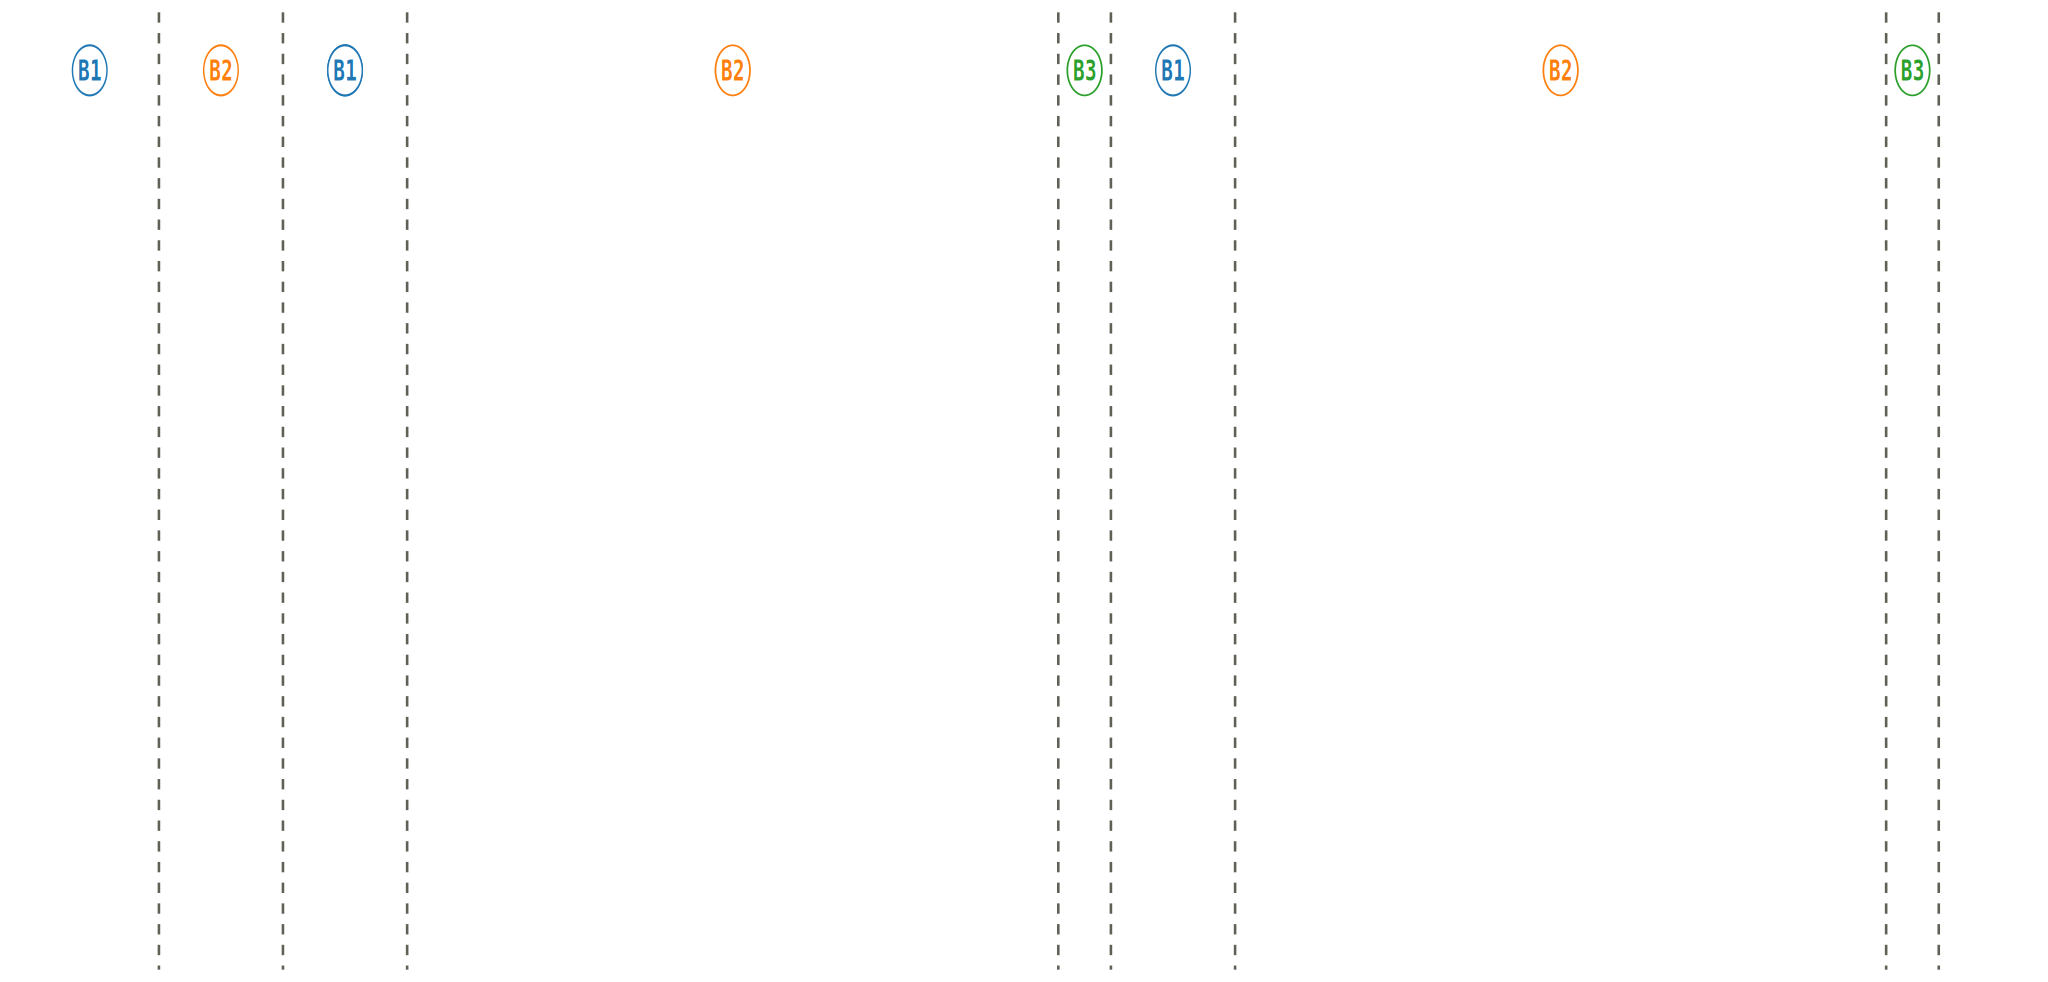
\includegraphics[width=\linewidth,height=6cm]{figures/behavior_bodytrack.pdf}
	\caption{\label{fig:case-study-bodytrack-medium}Phases de l'application \texttt{bodytrack-medium}}
\end{figure}

La bande passante vers la mémoire principale, le surcoût temporel observé, ainsi que le retard moyen par accès $D_{access}$ de chaque phase est montré dans la figure~\ref{fig:case-study-bodytrack-medium}.
Cette étude est intéressante à trois titres.
En premier lieu, on constate que les phases étiquetées avec le même comportement ont des bandes passantes et subissent un surcoût temporel presque identique.
Cela montre la pertinence du découpage effectué.
En deuxième lieu, on constate à nouveau le manque de précision de la caractérisation par la bande passante.
En effet, les phases avec les comportements $B_2$ et $B_3$, bien qu'ayant une bande passante presque identique, ont une sensibilité très différentes au problème d'interférences.
Le surcoût temporel observé pour $B_2$ et $B_3$ étant respectivement de 100\% et 20\% du temps d'exécution des phases. 
En troisième et dernier lieu, on constate que si $B_1$ et $B_3$ sont visuellements très similaires, les bandes passantes et le surcoût observé pour ces comportements ne le sont pas.
Par contre, le retard moyen subi par accès est presque identique\footnote{de manière équivalente, on peut noter sur la figure~\ref{fig:case_study} que les points des phases correspondant à ces comportements sont alignés avec l'origine.}.
Cela montre l'intérêt de la prise en compte des aspects qualitatifs dans la caractérisation du comportement d'accès à la mémoire.

% Elle illustre également le manque de précision d'une caractérisation purement quantitative.
% En effet, les comportements $B2$ et $B3$ ont une bande quasiment identique, mais ont des sensibilités très différents : les facteurs de ralentissement observé étant respectivement de 100\% et 20\%.
% Enfin, on peut observer dans la figure~\ref{bodytrack-medium} que les phases $B1$  $B3$ sont visuellement très similaires.
% Cette similarité n'est pas capturée par la bande passante ni le retard global.
% On la retrouve par contre dans le retard moyen subi par accès qui est presque identique pour ces deux phases.
% Ce qui montre l'intérêt de la prise en compte des critères qualitatifs.

\begin{figure}[ht!]
  \begin{subfigure}[t]{0.68\linewidth}
    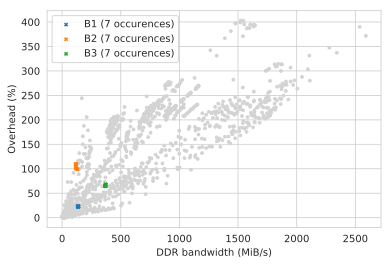
\includegraphics[width=\linewidth]{figures/bw_overhead_btrack.pdf}
    \caption{\label{fig:bw_ovd_btrack}}
  \end{subfigure}
  \begin{subfigure}[t]{0.3\linewidth}
    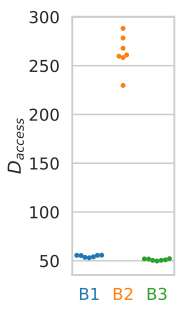
\includegraphics[width=\linewidth]{figures/phases_violin.pdf}
    \caption{\label{fig:phases_violin}}
  \end{subfigure}
	\caption{\label{fig:case_study} Sensibilité des différentes phases de l'application \texttt{bodytrack}}
\end{figure}


\section{Conclusions du chapitre}

Dans ce chapitre, nous avons abordé la caractérisation du comportement d'accès à la mémoire d'une application.
Les critères utilisés dans cette caractérisation devant être pertinents pour l'étude de la sensibilité aux phénomènes d'interférences mémoires.

Nous avons commencé par étudier le lien entre la bande passante (caractérisant l'intensité de l'activité mémoire) et le retard subi à cause des interférences.
D'une part, nous avons montré qu'il y effectivement une forte corrélation entre ces deux quantités : une bande passante élevée implique des retards importants.
D'autre part, nous avons montré que la plage de retards observés pour des bandes passantes presque identiques était très élevée, y compris pour des bandes passantes faibles.
Ainsi, la bande passante utilisée seule se révèle très imprécise pour caractériser la sensibilité aux interférences.

Afin de caractériser plus finement les comportements mémoires, nous avons introduit plusieurs \emph{métriques qualitatives} quantifiant des aspects liés à la nature du trafic.
Certaines de ces métriques n'étant pas directement mesurables au moyen de compteurs de performances, nous avons développé un outil de profilage permettant de les mesurer.
À l'aide de cet outil, nous pouvons distinguer des phases caractéristiques dans l'exécution d'applications.
Dans une étude de cas, nous avons montré que ces phases pouvaient être affectées très différemment par les interférences.

% Il est difficile d'évaluer tel quel la précision d'un mode de caractérisation.
% À plus forte raison, lorsque cette caractérisation dépends de plusieurs critères.
Dans la section suivante, nous allons juger de la pertinence des différentes métriques définies dans ce chapitre pour l'étude de la sensibilité aux interférences.
À cette fin, nous allons évaluer la précision qu'elles permettent d'atteindre lorsqu'elles sont utilisées pour l'inférence du retard causé par les interférences à des applications quelconques.
%Nous allons pour cela utiliser ces métriques pour inférer le retard subi par des applications en fonction de leur comportement en isolation.